\section{LoRa}\label{sec:etat_art-lora}
\renewcommand{\rightmark}{LoRa}

LoRa (Long Range)~\cite{sx1276:datasheet}\cite{paper:lora-reverse-engineering} est une technologie 
radio  fonctionnant sur une modulation propriétaire détenue par Semtech et basée sur \textit{chirp 
spread spectrum (CSS)}. \textit{chirp spread spectrum} consiste en un signal d'une amplitude 
constante pour lequel la fréquence diminue ou augmente au cours du temps. Ces variations qui sont 
pour LoRa linéaires, sont respectivement appelées \textit{downchirp} et \textit{upchirp}. Cette 
modulation permet d'obtenir des communications longues portées et basses énergie.

%\begin{wrapfigure}{r}{0.3\textwidth}
%    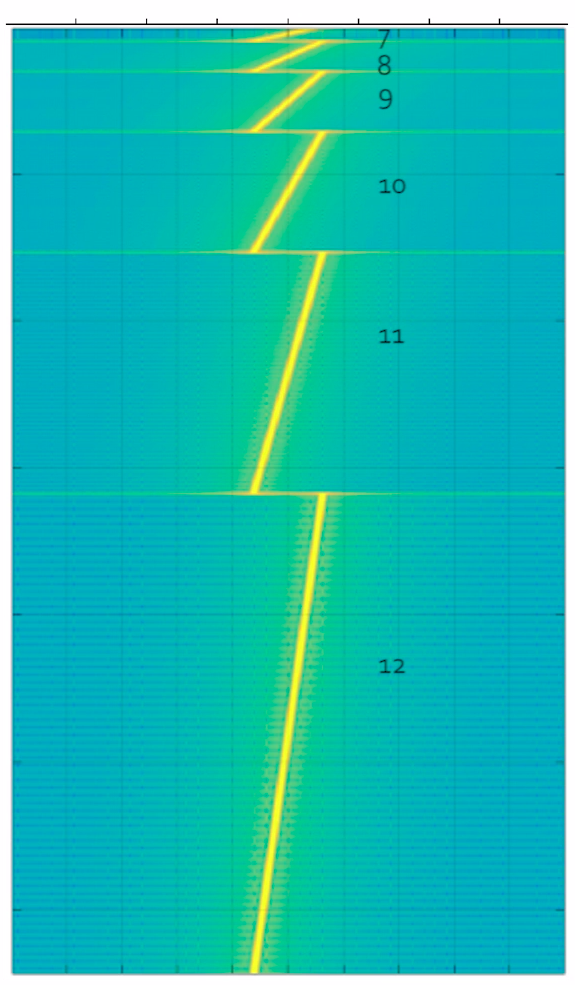
\includegraphics[scale=0.25]{res/pictures/lora-sf.png}
%    \caption{Signal en fonction du SF.\todo{ref}}
%    \label{fig:state-sf}
%\end{wrapfigure}
Une communication LoRa dépend des paramètres suivants:
\begin{itemize}
    \item \textbf{Spreading Factor (SF)} est une variable qui définit la vitesse de balayage du signal radio
    %i.e. le nombre chirps utilisés pour la transmission d'un symbole qui est $2^{SF}$
    (Fig~\ref{fig:state-sf}). Le spreading factor est compris entre 7 et 12. Plus sa valeur est grande, plus la vitesse de balayage est petite. Ceci implique un signal plus facile à décoder, mais avec un débit de données plus faible. Donc, inversement à une petite valeur de SF, une grande valeur de SF a un débit plus faible et une QoS (Quality of Service) plus élevée.
    
    \item \textbf{Bandwidth (BW)} détermine la largeur de la bande passante. Une bande passante plus large augmente la qualité du signal. Pour LoRa, en Europe, les valeurs de BW sont limitées à 125 KHz et 250KHz~\cite{lora-frequencyplan}.
    
    \item \textbf{Coding rate (CR)} détermine la quantité de bits redondants ajoutés par le codage 
    d'erreur cyclique utilisé par LoRa pour la détection et la correction d'erreurs. Cette méthode 
    de correction d'erreur permet au signal de supporter de courtes interférences. Ainsi, il est
    possible de coder des données de 4 bits avec des redondances de 5, 6, 7 ou 8 bits. La valeur du 
    CR se note donc 4/5, 4/6, 4/7 ou 4/8.
    
\end{itemize}

\begin{figure}[H]
    \centering
    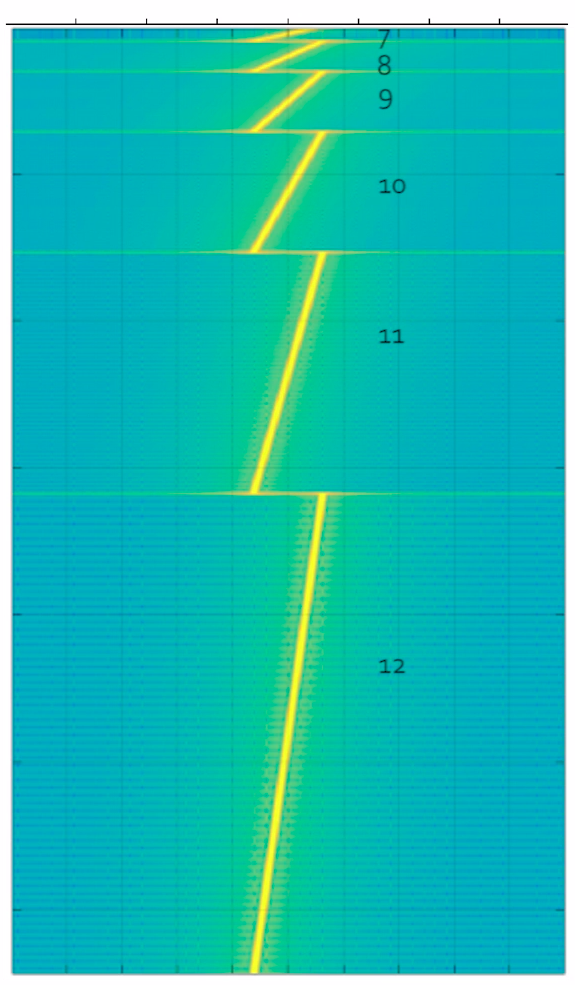
\includegraphics[scale=0.25]{res/pictures/lora-sf.png}
    \caption{Spectogramme des différents Spreading Factors~\cite{ghoslya}.}
    \label{fig:state-sf}
\end{figure}


%La relation entre SF et BW est décrite par l'équation~\ref{eq:state-lora-rs}.
%\begin{equation}\label{eq:state-lora-rs}
%    Rs = \frac{BW}{2^{SF}}
%\end{equation}

\vspace{1cm}
Le format des paquets LoRa (Fig.~\ref{fig:state-lora-frame-format}) peut être explicite ou implicite.
Dans le mode implicite, le header n'est pas inclus dans le paquet. Pour cela, la taille de la payload, le coding rate et la présence de la Payload CRC (Cyclic Redundancy Check) doivent être configurés.
Ce mode permet de réduire la taille du paquet et donc du temps de transmission.

\begin{figure}[H]
    \centering
    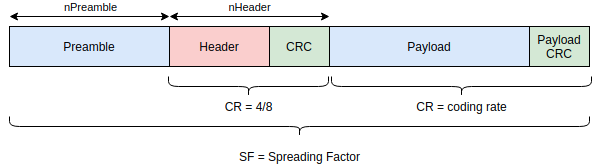
\includegraphics[scale=0.6]{res/pictures/lora-frame-format.drawio.png}
    \caption{Format d'un paquet LoRa.}
    \label{fig:state-lora-frame-format}
\end{figure}

La datasheet du SX1276 intégré dans le RN2383, utilisé comme transceiver LoRa pour ce projet (c.f.~\ref{hardware:rn2483}), définit le temps d'émission d'un paquet LoRa reprit par l'équation~\ref{eq:state-lora-tframe}.
\begin{equation}\label{eq:state-lora-tframe}
    T_{frame} = T_{preamble} + T_{payload}
\end{equation}

Où $T_{preamble}$ et $T_{payload}$ sont respectivement le temps d'émission du preamble et du payload définis aux équations \ref{eq:state-lora-tpreamble} et \ref{eq:state-lora-tpayload}.

\begin{equation}\label{eq:state-lora-tpreamble}
    T_{preamble} = (n_{preamble} + 4,25)T_{sym}
\end{equation}

\begin{equation}\label{eq:state-lora-tpayload}
    T_{payload} = n_{payload} * T_{sym}
\end{equation}

Où $T_{sym} = \frac{1}{R_s}$, $n_{preamble}$ et $n_{payload}$ sont le nombre de symboles du preamble et du payload. $n_{preamble}$ est une valeur paramétrable du module radio et $n_{payload}$ est défini par l'équation~\ref{eq:state-lora-npayload}.

\begin{equation}\label{eq:state-lora-npayload}
    \begin{split}
    n_{payload} =8 +max
     \left( ceil \left[ \frac{8PL - 4SF + 28 + 16CRC - 20IH}{4(SF-2DE)} \right] (CR+4), 0 \right)
    \end{split}
\end{equation}

où:
\begin{itemize}
    \item $PL$ est le nombre d'octets de la payload (1 à 255)
    \item $SF$ est le spreading factor
    \item $CRC=1$ si une CRC est présente $CRC=0$ sinon
    \item $IH=0$ si le header est présent, $IH=1$ sinon
    \item $DE=1$ si $LowDataRateOptimize=1$, $DE=0$ sinon.\\
    $LowDataRateOptimize$ permet d'optimiser la robustesse d'une transmission quand celle-ci est longue.
    \item $CR$ prend la valeur 1 pour $4/5$, 2 pour $4/6$, etc
\end{itemize}
\vspace{0.5cm}
Cette dernière équation permet les déductions suivantes:
\begin{itemize}
    \item Il y a toujours au minimum 8 symboles
    \item Le numérateur de la fraction quantifie un nombre de bits car PL est multiplié par 8
    \item La CRC a une taille de 16 bits
    \item Le header a une taille de 20 bits
\end{itemize}